\section {The NFActor Framework}

\begin{figure}[!t]
  \centering
  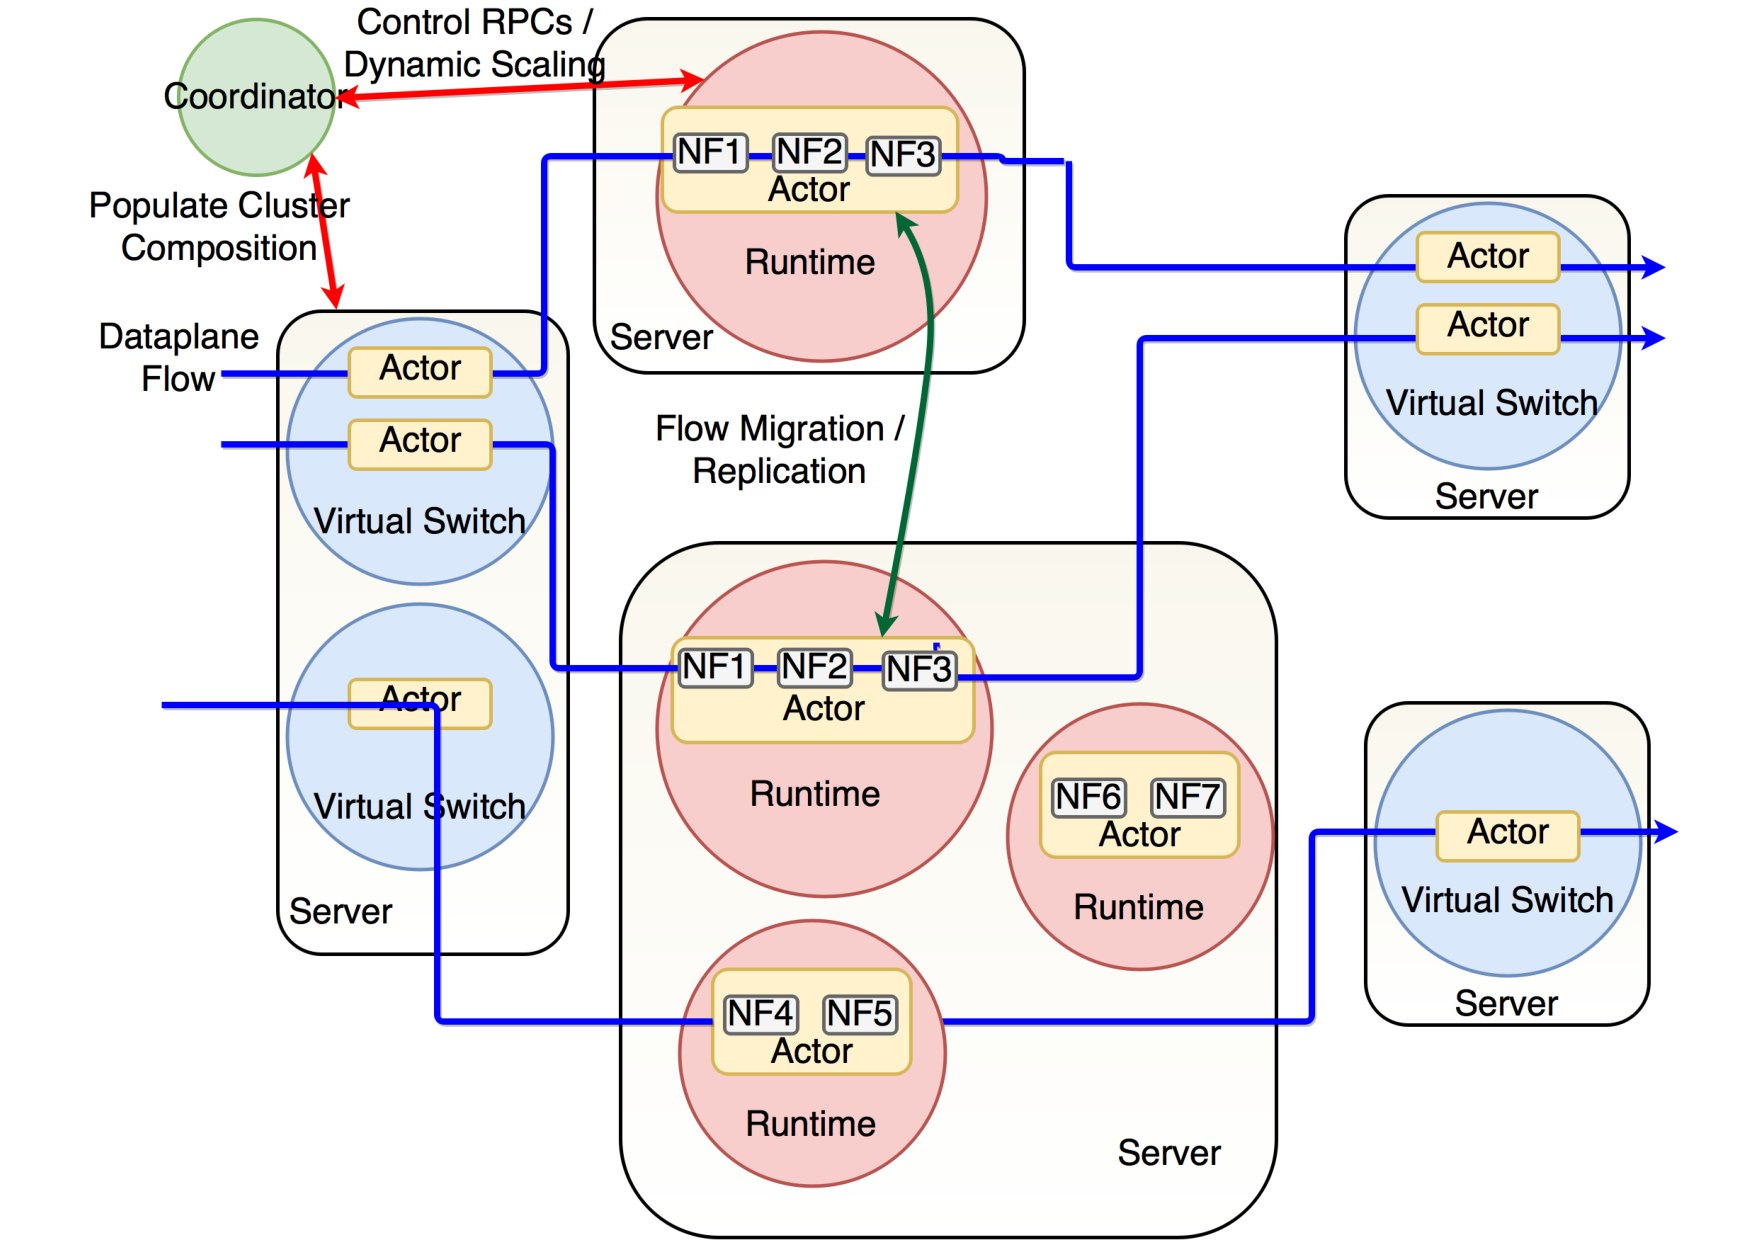
\includegraphics[width=\columnwidth]{figure/new-nfactor-cluster.pdf}
  \caption{An overview of \nfactor.}
  \label{fig:runtime}
\end{figure}

We first present key design and modules in \nfactor.

\subsection{Overview}
\label{sec:overview}

\nfactor~includes three modules: (i) runtime systems that enable flow processing using actors; (ii) virtual switches for distributing flows to runtime systems and sending flows to final destinations; and (iii) a lightweight coordinator for basic system management. % (\eg, runtime load monitoring and scaling, participate in the initiation phase of flow migration and replication).
 An illustration of the \nfactor~system is given in Fig.~\ref{fig:runtime}.

A runtime system, referred to as \textit{runtime} for short, is the execution environment of service chains. A runtime is running on a container, for quick launching and rebooting in cases of scaling out/in and failure recovery. There can be multiple runtimes (containers) running on the same physical server. In \nfactor, the virtual switches are running in the same environments (containers) as those runtimes, % and run actors for flow distribution, 
 \ie, they can be regarded as special runtimes. % running a load balancer function. 
 Runtimes and virtual switches are connected through a L2 network.

%When a dataplan flow arrives in the system, it is first sent to a virtual switch.
Each virtual switch is configured with an entry IP address. The coordinator sets up flow rules to direct dataplane flows to virtual switches, which further dispatch them to runtimes hosting respective service chains. A runtime creates a dedicated flow actor for processing each flow. After processing, the outgoing flow packets are sent to another virtual switch,
%(which can be the same or a different virtual switch where the flow comes into the system),
which forwards the flow to its final destination.\footnote{When our flow replication mechanism is in place, the flow will be sent by the replica runtime to the virtual switch, to be further forwarded outside (Sec.~\ref{sec:resilience}).}



%The key feature that differentiates NFActor framework from the existing works like \cite{gember2015opennf} and \cite{rajagopalan2013split} is that, resilience operations, \ie~flow migration and replication, is fully decentralized. Figure \ref{fig:runtime} demonstrates a flow migration process that migrates actor 2 on runtime 1 to runtime 2. \ac{The migration starts by actor 2 sending the first request to runtime 2. Runtime 2 launches actor 4, which is used as the migration target actor for accepting the flow packets and flow states of actor 2, before responding to actor 2. Actor 2 then sends the second request to the virtual switch, asking it to modify the output route to runtime 2. Finally, actor 2 sends its flow states in the third request to actor 4, completing the whole migration process. The details of our distributed flow migration is further illustrated in \ref{}.} \cui{The third paragraph on describing flow migration is not clear. Should make it more clear, or make it the "Section 3.1 Example" section, or cut this paragraph.}

%our main observration is that actor privdes the unique feature to implement a high throughput system due to its light-weight execution state and and

%%%light-weight, decentralized migration of network flow states

%Our main observation is that actor provides the unique benefits for light-weight, decentralized migration of network flow states.

The design of \nfactor~targets the following goals. %\chuan{complete the following. each bullet 2-3 sentences}

{\bf Transparent Resilience.}  Flow migration and replication operations, those needed to enable failure resilience, are carried out transparently to flow processing through any service chain, in largely distributed fashion.

%Flow actor should be able to transparently perform resilience operations, including flow migration and replication, regardless of the service chain that is configured for it. %The NF modules implemented using the module API (Sec.~\ref{sec:module-api}) should be transparently

{\bf High Scalability.} Good horizontal scalability is achieved for runtimes and virtual switches, so that~\nfactor adopts to varying workload timely with ease.

{\bf High Packet Processing Throughput.} Extra overhead for flow migration, replication, and system scaling is minimized, to ensure high-speed packet processing.
